%%%%%%%%%%%%%%%%%%%%%%%%%%%%%%%%%%%%%%%%%%%%%%%%%%%%%%%%%%%%%%%%%%%%%%
%%%%%%%%%%%%%%%%%%%%%%%%%%%%%%%%%%%%%%%%%%%%%%%%%%%%%%%%%%%%%%%%%%%%%%
\documentclass[dvips,portrait]{seminar}             %%%%%%%%%%%%%%%%%%
                                                    %%%%%%%%%%%%%%%%%%
%%%%%%%%%%%%%%%%%%%%%%%%%%%%%%%%%%%%%%%%%%%%%%%%%%%%
% gmake afb-ang-ps
%======================

\input Energy.tex
\def\Energy{MZ-1.8GeV (had.)}
\def\Angle{$\theta^{\bullet}$}


%%%%%%%%%%%%%%%%%%%%%%%%%%%%%%%%%%%%%%%%%%%%%%%%%%%%%%%
%%%%%%%%%%%%%%%%%%%%%%%%%%%%%%%%%%%%%%%%%%%%%%%%%%%%%%%
\begin{document}                     %%%%%%%%%%%%%%%%%%

%%%%%%%%%%%%%%%%%%%%%%%%%%%%%%%%%%%%%%%%%%%%%%%%%%%%%%%%%%%%%%%%%%%%%%%%%%%%%
%%%%%%%%%%%%%%%%%%%%%%%%%%%%%%%%%%%%%%%%%%%%%%%%%%%%%%%%%%%%%%%%%%%%%%%%%%%%%
%%%%%%%%%%%%%%%%%%%%%%%%%%%%%%%%%%%%%%%%%%%%%%%%%%%%%%%%%%%%%%%%%%%%%%%%%%%%%
                                                         %%%%%%%%%%%%%%%%%%%%
\begin{slide*}
\titbox{{\small\Color{Magenta} 
      ISR*FSR interf. in angular distribution}}

{\small\Color{Blue}
  The influence of ISR*FSR  interference at \Energy. 
  The energy cut is on $s'/s$, where $s'=m^2_{f\bar{f}}$.
  The angular cut is $|\cos\theta|<\cos\theta_{\max}$}
{\small\Color{Blue} Scattering angle is $\theta=$\Angle. }
{\tiny\Color{Blue}  [Angle $\theta^{\bullet}$ is defined in Phys. Rev. {\bf D41}, 1425 (1990)]}

%-----------------------------------------------------------
\begin{center}
\setlength{\unitlength}{1mm}
%
\begin{picture}(35,35)
\put(-1, 0){\makebox(0,0)[lb]{
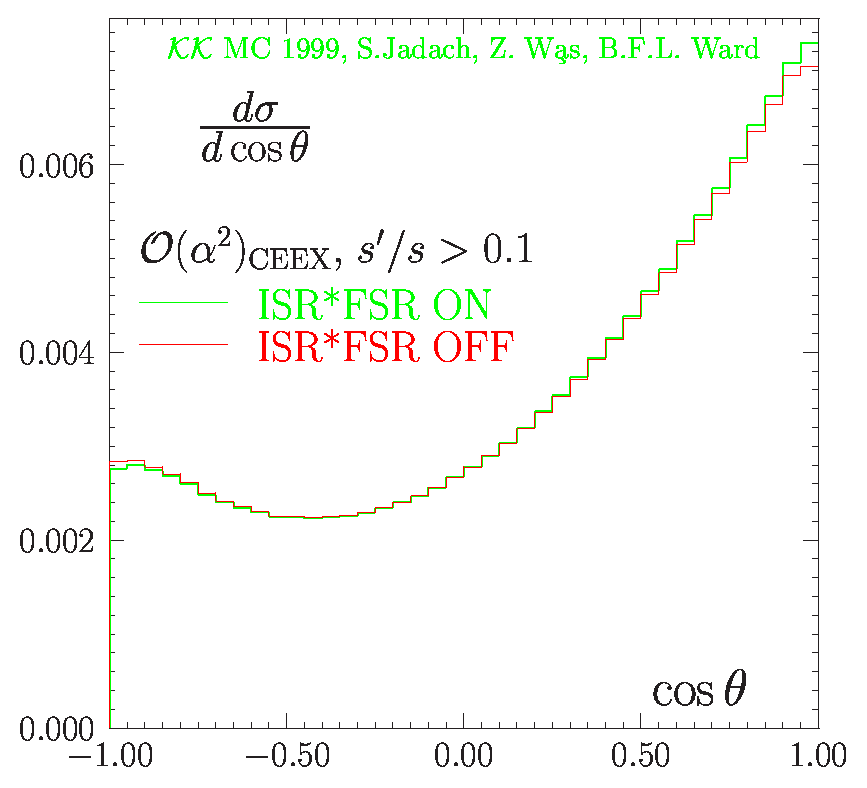
\epsfig{file=afb-int-G1.eps,width=35mm,height=34mm}
}}\end{picture}
%
\begin{picture}(35,35)
\put(-1, 0){\makebox(0,0)[lb]{
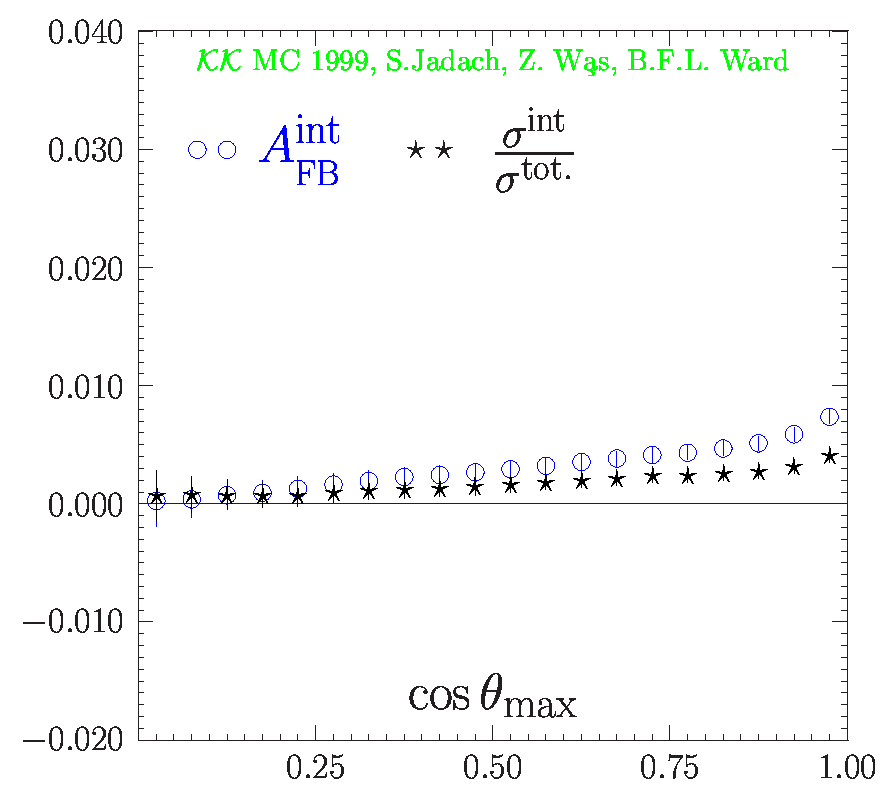
\epsfig{file=afb-int-com1.eps,width=35mm,height=34mm}
}}\end{picture}
%
\end{center}
%-----------------------------------------------------------
\begin{center}
\setlength{\unitlength}{1mm}
%
\begin{picture}(35,35)
\put(-1, 0){\makebox(0,0)[lb]{
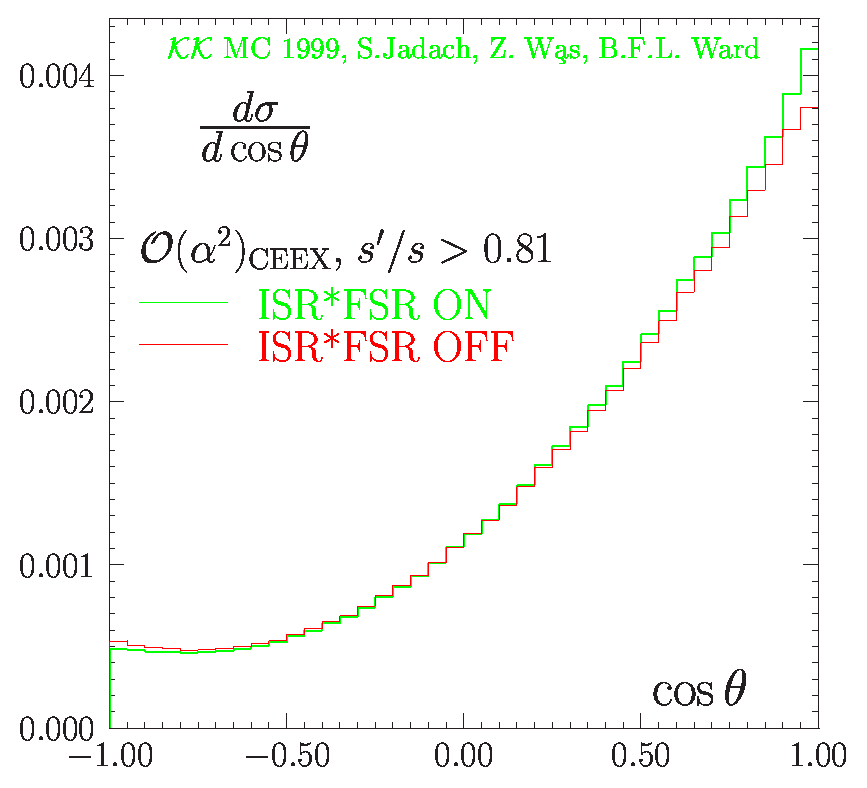
\epsfig{file=afb-int-G1x.eps,width=35mm,height=34mm}
}}\end{picture}
%
\begin{picture}(35,35)
\put(-1, 0){\makebox(0,0)[lb]{
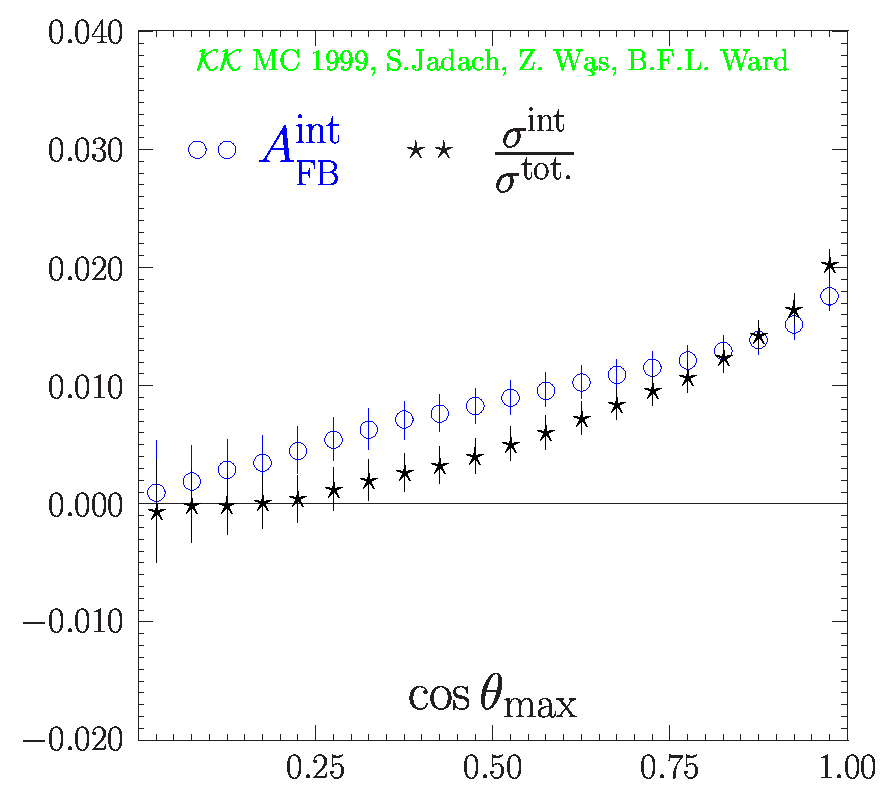
\epsfig{file=afb-int-com1x.eps,width=35mm,height=34mm}
}}\end{picture}
%
\end{center}
%-----------------------------------------------------------
\vfill
\end{slide*}   %%%
%%%%%%%%%%%%%%%%%%



%%%%%%%%%%%%%%%%%%%%%%%%%%%%%%%%%%%%%%%%%%%%%%%%%%%%%%%%%%%%%%%%%%%%%%%%%%%%%
%%%%%%%%%%%%%%%%%%%%%%%%%%%%%%%%%%%%%%%%%%%%%%%%%%%%%%%%%%%%%%%%%%%%%%%%%%%%%
%%%%%%%%%%%%%%%%%%%%%%%%%%%%%%%%%%%%%%%%%%%%%%%%%%%%%%%%%%%%%%%%%%%%%%%%%%%%%
                                                         %%%%%%%%%%%%%%%%%%%%
\begin{slide*}
\titbox{{\small\Color{Magenta} 
      ISR*FSR interf. Realistic acceptance}}

{\small\Color{Blue}
  The influence of ISR*FSR  interference at \Energy. 
  The energy cut is on $v_p=1-Q^2_{Aleph}/s$, where $Q^2_{Aleph}$ 
  is s-channel propagator variable of ALEPH.
  The angular cut is $|\cos\theta|<\cos\theta_{\max}$}
{\small\Color{Blue} Scattering angle is $\theta=$\Angle. }
{\tiny\Color{Blue}  [Angle $\theta^{\bullet}$ is defined in Phys. Rev. {\bf D41}, 1425 (1990)]}

%-----------------------------------------------------------
\begin{center}
\setlength{\unitlength}{1mm}
%
\begin{picture}(35,35)
\put(-1, 0){\makebox(0,0)[lb]{
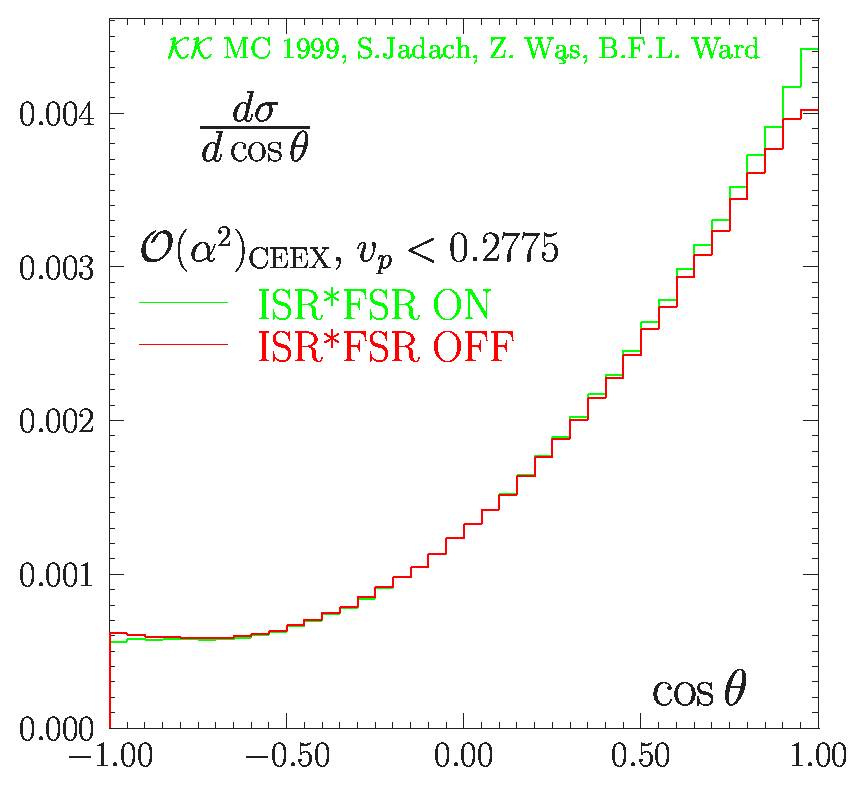
\epsfig{file=afb-int-G1xxx.eps,width=35mm,height=34mm}
}}\end{picture}
%
\begin{picture}(35,35)
\put(-1, 0){\makebox(0,0)[lb]{
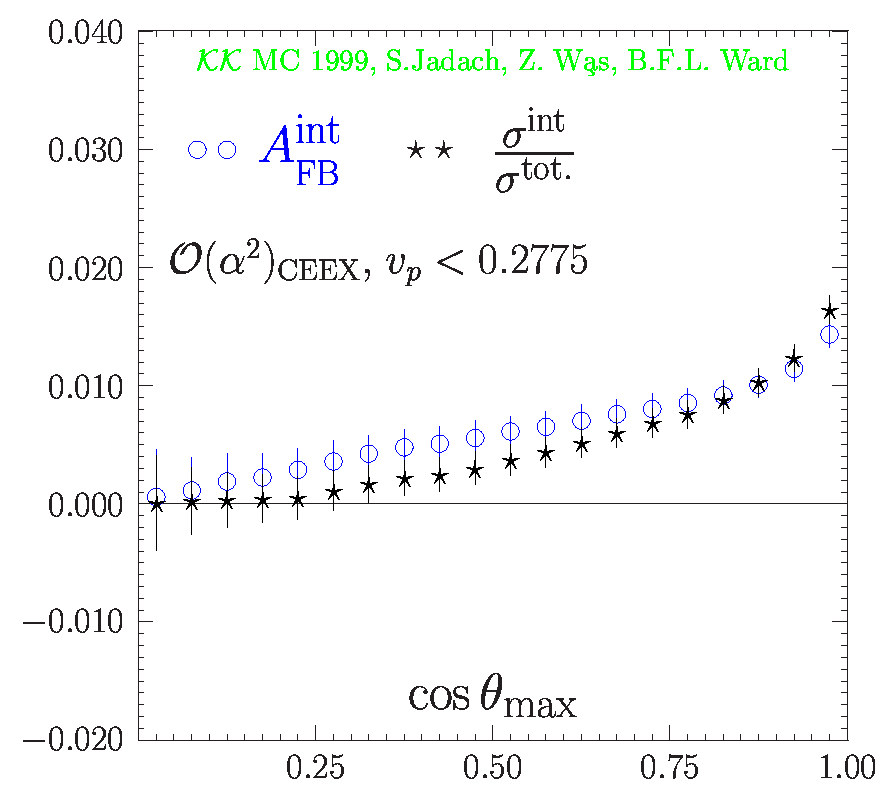
\epsfig{file=afb-int-com1xxx.eps,width=35mm,height=34mm}
}}\end{picture}
%
\end{center}
%-----------------------------------------------------------
\vfill
\end{slide*}   %%%
%%%%%%%%%%%%%%%%%%





%%%%%%%%%%%%%%%%%%%%%%%%%%%%%%%%%%%%%%%%%%%%%%%%%%%%%%%%%%%%%%%%%%%%%%%%%%%%%
%%%%%%%%%%%%%%%%%%%%%%%%%%%%%%%%%%%%%%%%%%%%%%%%%%%%%%%%%%%%%%%%%%%%%%%%%%%%%
%%%%%%%%%%%%%%%%%%%%%%%%%%%%%%%%%%%%%%%%%%%%%%%%%%%%%%%%%%%%%%%%%%%%%%%%%%%%%
                                                         %%%%%%%%%%%%%%%%%%%%
\begin{slide*}
\titbox{{\small\Color{Magenta} 
      ISR*FSR interf. Realistic acceptance}}

{\small\Color{Blue}
  The influence of ISR*FSR interference at \Energy. 
  The energy cut is on $v_p=1-Q^2_{Aleph}/s$, where $Q^2_{Aleph}$ 
  is s-channel propagator variable of ALEPH.
  No angular cut.}
%-----------------------------------------------------------
\begin{center}
\setlength{\unitlength}{1mm}
%
\begin{picture}(35,35)
\put(-1, 0){\makebox(0,0)[lb]{
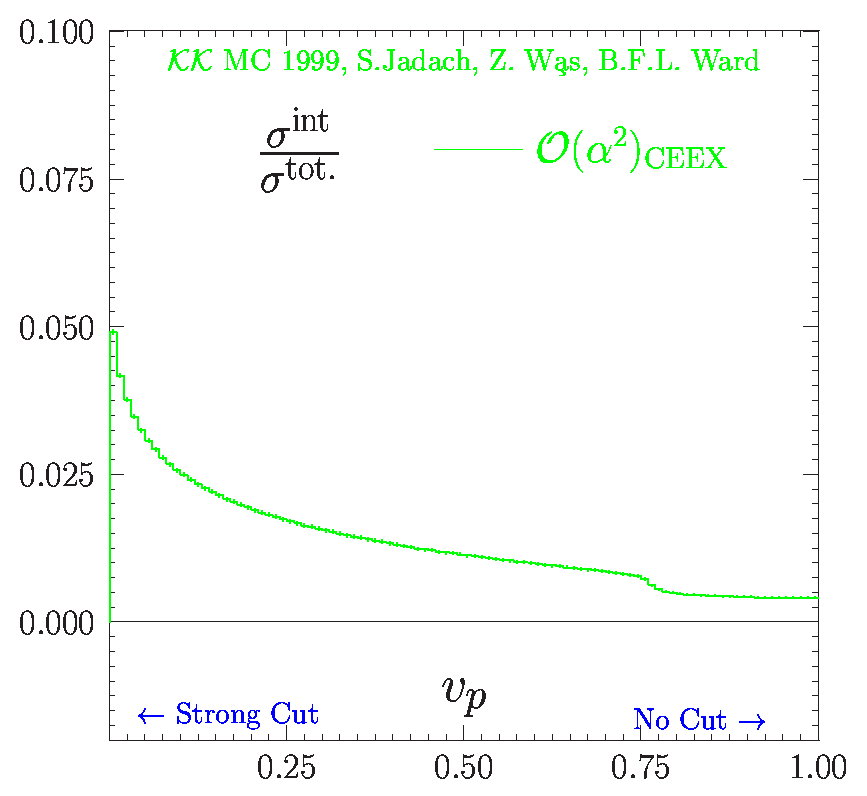
\epsfig{file=afb-int-sig1S.eps,width=35mm,height=34mm}
}}\end{picture}
%
\begin{picture}(35,35)
\put(-1, 0){\makebox(0,0)[lb]{
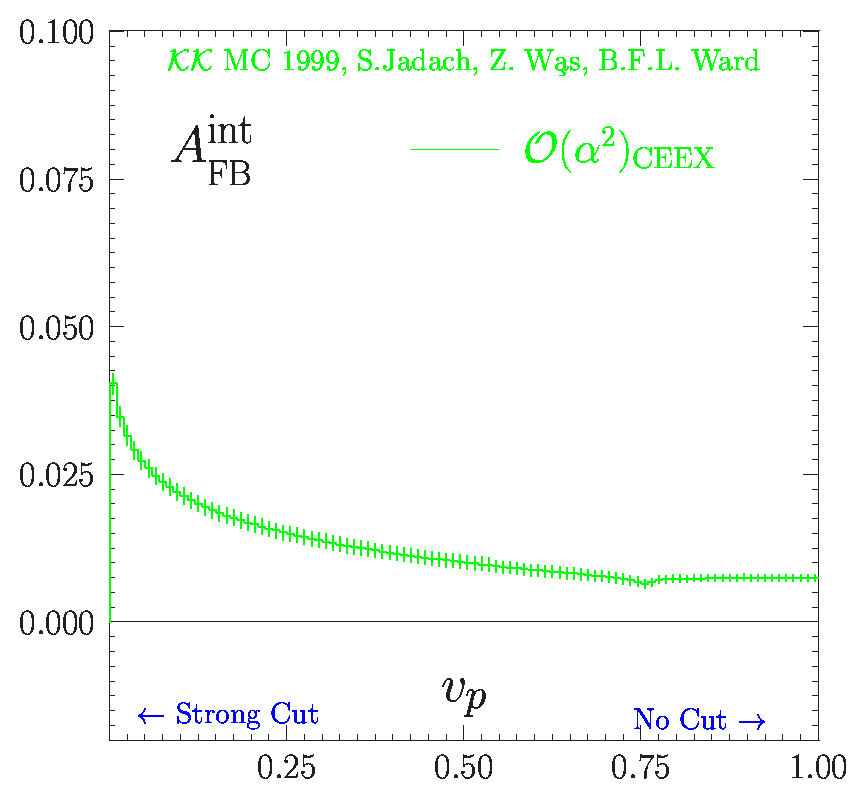
\epsfig{file=afb-int-afb1S.eps,width=35mm,height=34mm}
}}\end{picture}
%
\end{center}
%-----------------------------------------------------------
\vfill
\end{slide*}   %%%
%%%%%%%%%%%%%%%%%%






%%%%%%%%%%%%%%%%%%%%%%%%%%%%%%%%%%%%%%%%%%%%%%%%%%%%%%%%%%%%%%%%%%%%%%%%%%%%%
%%%%%%%%%%%%%%%%%%%%%%%%%%%%%%%%%%%%%%%%%%%%%%%%%%%%%%%%%%%%%%%%%%%%%%%%%%%%%
%%%%%%%%%%%%%%%%%%%%%%%%%%%%%%%%%%%%%%%%%%%%%%%%%%%%%%%%%%%%%%%%%%%%%%%%%%%%%
                                                         %%%%%%%%%%%%%%%%%%%%
\begin{slide*}
\titbox{{\small\Color{Magenta} 
      ISR*FSR interf. KORALZ 1-st order}}

{\small\Color{Blue}
  The influence of ISR*FSR  interference at \Energy. 
  The energy cut is on $s'/s$, where $s'=m^2_{f\bar{f}}$.
  The angular cut is $|\cos\theta|<\cos\theta_{\max}$}
{\small\Color{Blue} Scattering angle is $\theta=$\Angle. }
{\tiny\Color{Blue}  [Angle $\theta^{\bullet}$ is defined in Phys. Rev. {\bf D41}, 1425 (1990)]}

%-----------------------------------------------------------
\begin{center}
\setlength{\unitlength}{1mm}
%
\begin{picture}(35,35)
\put(-1, 0){\makebox(0,0)[lb]{
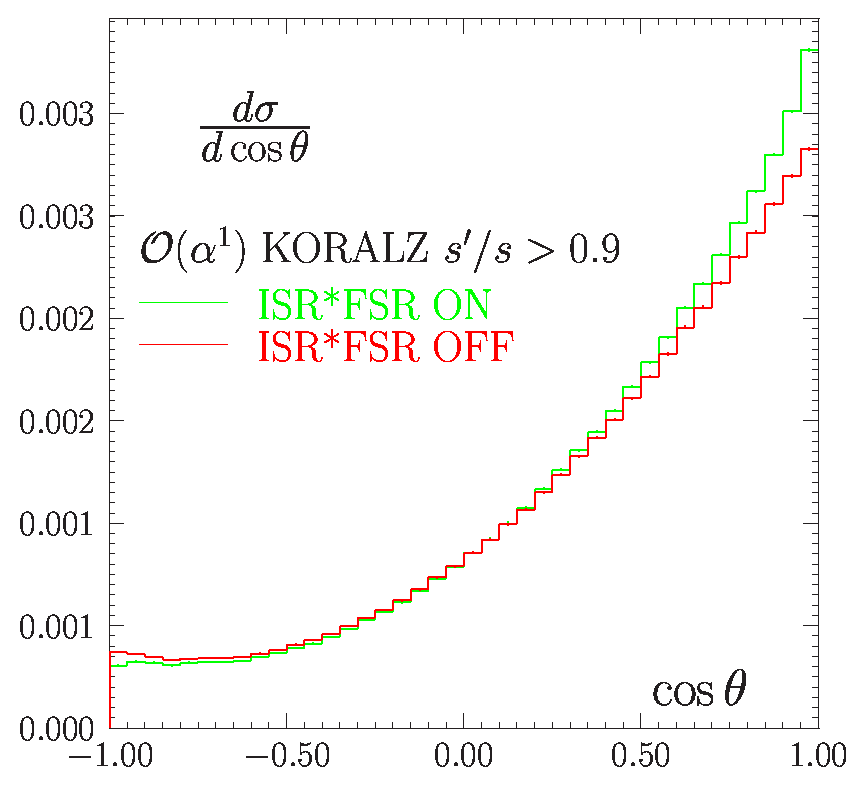
\epsfig{file=afb-int-AngMx.eps,width=35mm,height=34mm}
}}\end{picture}
%
\begin{picture}(35,35)
\put(-1, 0){\makebox(0,0)[lb]{
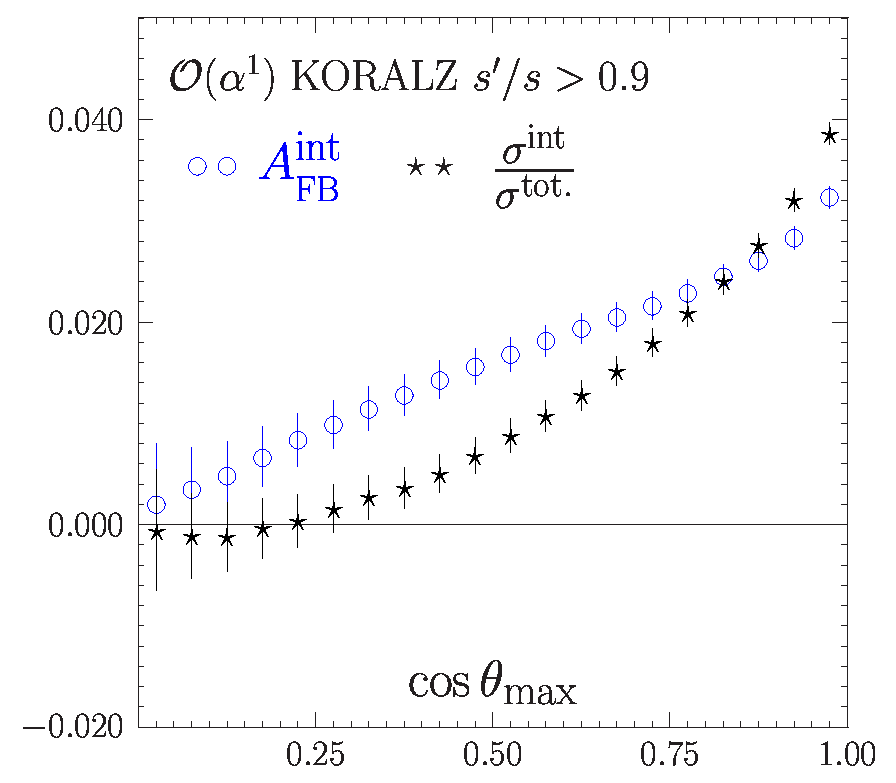
\epsfig{file=afb-int-comMx.eps,width=35mm,height=34mm}
}}\end{picture}
%
\end{center}
%-----------------------------------------------------------
\vfill
\end{slide*}   %%%
%%%%%%%%%%%%%%%%%%






\end{document}                                           %%%%%%%%%%%%%%%%%%%%
%%%%%%%%%%%%%%%%%%%%%%%%%%%%%%%%%%%%%%%%%%%%%%%%%%%%%%%%%%%%%%%%%%%%%%%%%%%%%
%%%%%%%%%%%%%%%%%%%%%%%%%%%%%%%%%%%%%%%%%%%%%%%%%%%%%%%%%%%%%%%%%%%%%%%%%%%%%
%%%%%%%%%%%%%%%%%%%%%%%%%%%%%%%%%%%%%%%%%%%%%%%%%%%%%%%%%%%%%%%%%%%%%%%%%%%%%
%%%%%%%%%%%%%%%%%%%%%%%%%%%%%%%%%%%%%%%%%%%%%%%%%%%%%%%%%%%%%%%%%%%%%%%%%%%%%

